% Derivative of tangent from the unit circle: t = tan(theta) is the vertical side
% of a right triangle with base 1 and hypotenuse L = sec(theta). Rotating by
% dtheta sweeps the corner through L*dtheta, and dividing that leg by cos(theta)
% gives dt = L*dtheta/cos(theta) = sec^2(theta) dtheta.
\ifnum\pdfoutput>0
  \documentclass[tikz,border=3pt]{standalone}         % pdflatex → PDF proof
\else
  \documentclass[tikz,border=3pt,dvisvgm]{standalone} % latex   → web SVG
\fi
% Shared setup for all site figures — \input by every figures/*.tex.
% Change the palette, font size, or driver logic HERE and every figure inherits
% it on next rebuild. See src/assets/blog/README.md for the full workflow.
%
% NOTE: this file is \input AFTER \documentclass (it needs amsmath/tikz loaded),
% but the \documentclass line itself carries the driver switch and must stay in
% each figure — see _template.tex. Keep figure .tex files starting from that
% template so the driver logic is never forgotten.

\usepackage{amsmath}

% --- Palette: sentinel hexes = the LIGHT-theme values from DESIGN.md. ----------
% The PDF proof / Overleaf output therefore look like the light rendering, and
% fig.sh rewrites each hex to its themed CSS variable in the web SVG:
%   ink    #000000 -> var(--color-text-main, currentColor)   (also all black strokes)
%   accent #003366 -> var(--color-accent, #003366)
%   muted  #555555 -> var(--color-text-muted, #555555)
%   figred #b91c1c -> var(--fig-red, #b91c1c)
%   figblue   #1d4ed8 -> var(--fig-blue, #1d4ed8)
%   figorange #c2410c -> var(--fig-orange, #c2410c)
\definecolor{ink}{HTML}{000000}
\definecolor{accent}{HTML}{003366}
\definecolor{muted}{HTML}{555555}
\definecolor{figred}{HTML}{B91C1C}
\definecolor{figblue}{HTML}{1D4ED8}
\definecolor{figorange}{HTML}{C2410C}

% --- Figure body font size = site body text. ---------------------------------
% The site renders body text at 18px ≈ 13.5pt. dvisvgm emits the SVG at its
% intrinsic point size and <Figure> shows it ~1:1, so to make figure labels match
% surrounding prose we set the figure's \normalsize to 13.5/16pt. Individual
% labels can still deviate with font=\small / font=\large as needed. Computer
% Modern matches the KaTeX body math, so $dg_p(v)$ reads identically in both.
\newcommand{\figfontsize}{\fontsize{13.5}{16}\selectfont}

% Apply it as the default font for every tikzpicture, plus sane global defaults.
% Dimension figures in mm (x=1mm,y=1mm) so geometry and this pt-based text stay
% independent — scale the drawing by editing coordinates, not the type size.
\tikzset{
  every picture/.style = {font=\figfontsize, line join=round},
  edge/.style          = {line width=1pt},
  hair/.style          = {line width=1pt},
}


\begin{document}
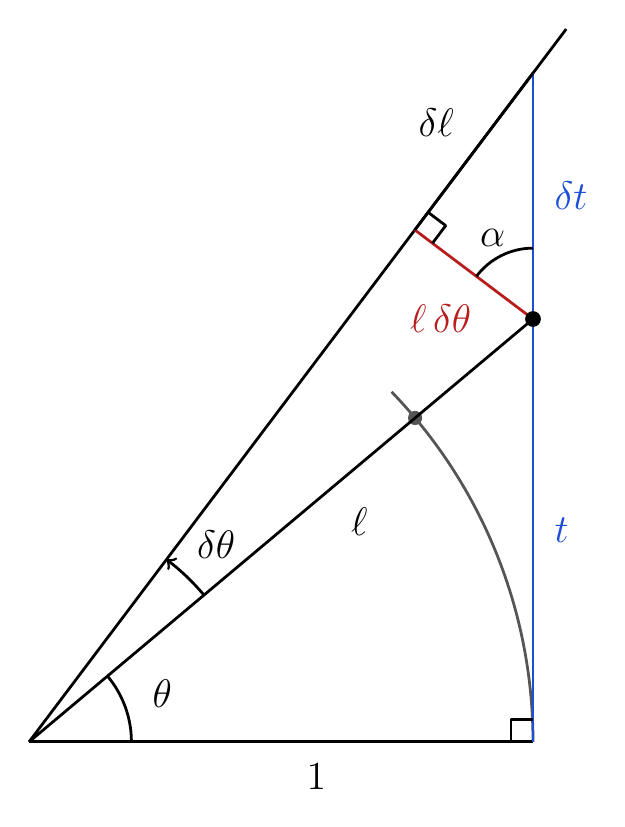
\begin{tikzpicture}[x=1mm, y=1mm]
  \def\U{64}\def\Th{40}\def\dTh{13}    % base (= 1), angle, angular nudge

  \pgfmathsetmacro{\Lh}{\U/cos(\Th)}          % hypotenuse, sec(theta)
  \pgfmathsetmacro{\Tt}{\U*tan(\Th)}          % t = tan(theta)
  \pgfmathsetmacro{\Tq}{\U*tan(\Th+\dTh)}     % t + dt
  \pgfmathsetmacro{\Fx}{\Lh*cos(\dTh)*cos(\Th+\dTh)}   % foot of the perpendicular
  \pgfmathsetmacro{\Fy}{\Lh*cos(\dTh)*sin(\Th+\dTh)}   % dropped from P onto the
  \pgfmathsetmacro{\Mx}{(\U+\Fx)/2}                    % nudged ray, and the
  \pgfmathsetmacro{\My}{(\Tt+\Fy)/2}                   % midpoint of that leg

  \coordinate (O) at (0,0);
  \coordinate (A) at (\U,0);
  \coordinate (P) at (\U,\Tt);
  \coordinate (Q) at (\U,\Tq);
  \coordinate (F) at (\Fx,\Fy);

  % the unit circle this triangle is built on, kept faint
  \draw[hair, muted] (0:\U) arc[start angle=0, end angle={\Th+4}, radius=\U];
  \fill[muted] (\Th:\U) circle (0.9);

  \draw[edge, ink]  (O) -- (A);
  \draw[edge, ink]  (O) -- (P);
  \draw[hair, ink]  (O) -- ({\Th+\dTh}:{\U/cos(\Th+\dTh)+7});   % out past the corner Q
  \draw[edge, figblue] (A) -- (Q);
  \draw[edge, figred]  (P) -- (F);
  \draw[edge, ink]     (F) -- (Q);   % third side: the growth of the hypotenuse
  \fill[ink] (P) circle (1);

  % right angles: at the foot of the perpendicular, and at the base
  \draw[hair, ink] (F) ++({\Th+\dTh-90}:2.8) -- ++({\Th+\dTh}:2.8) -- ++({\Th+\dTh+90}:2.8);
  \draw[hair, ink] (A) ++(-2.8,0) -- ++(0,2.8) -- ++(2.8,0);

  % theta and its nudge at the origin
  \draw[hair, ink] (0:13) arc[start angle=0, end angle=\Th, radius=13];
  \node[ink] at ({\Th/2}:18) {$\theta$};
  \draw[hair, ink, ->] (\Th:29) arc[start angle=\Th, end angle={\Th+\dTh}, radius=29];
  \node[ink] at ({\Th+\dTh/2}:34.5) {$\delta\theta$};

  % the angle inside the small triangle: exactly theta + dtheta, so it gets its
  % own name rather than being called theta
  \draw[hair, ink] ([shift=(90:9)]P) arc[start angle=90, end angle={90+\Th+\dTh}, radius=9];
  \node[ink] at ([shift={({90+(\Th+\dTh)/2}:11.5)}]P) {$\alpha$};

  % right of the true midpoint on purpose: the theta arc lands on the base and
  % eats its left end, so a centered label reads as sitting left of center
  \node[below, text=ink] at ({0.57*\U},-1.5) {$1$};
  \node[ink] at ({0.6*\Lh*cos(\Th)+5.5*cos(\Th-90)},{0.6*\Lh*sin(\Th)+5.5*sin(\Th-90)}) {$\ell$};
  \node[right, text=figblue] at ({\U+1.5},{\Tt/2}) {$t$};
  \node[right, text=figblue] at ({\U+1.5},{(\Tt+\Tq)/2}) {$\delta t$};
  % dL sits on the outer side of its own segment, pushed out along the normal
  \node[ink] at ({(\Fx+\U)/2+6*cos(\Th+\dTh+90)},{(\Fy+\Tq)/2+6*sin(\Th+\dTh+90)}) {$\delta\ell$};
  % leg label: midpoint of the perpendicular, pushed out along its own normal
  \node[text=figred] at ({\Mx+7*cos(\Th+\dTh+180)},{\My+7*sin(\Th+\dTh+180)}) {$\ell\,\delta\theta$};
\end{tikzpicture}
\end{document}
